\section{Results}

\subsection{Transformation Functions} 

\begin{figure}[H]
    \centering
    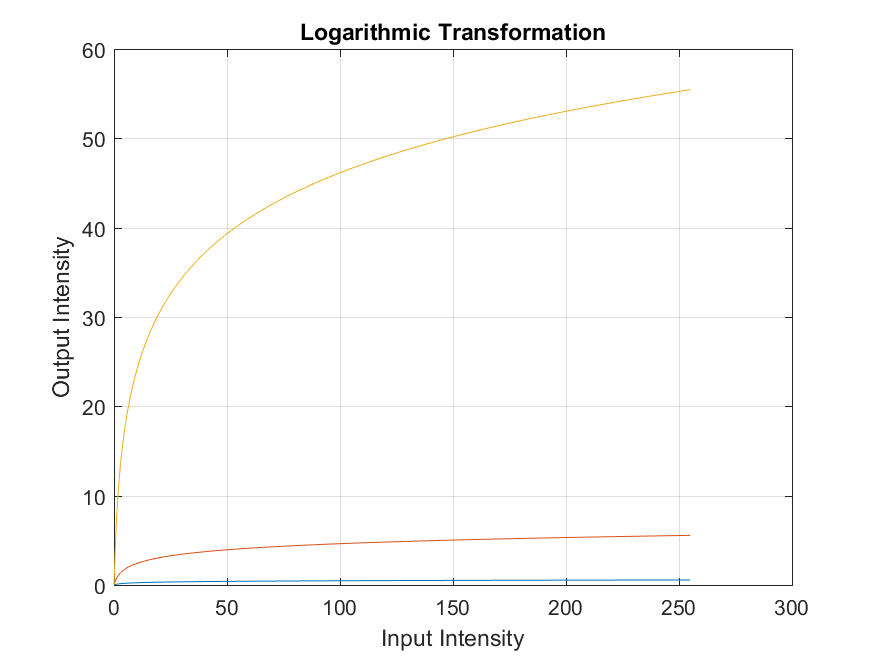
\includegraphics{logarithmic}
    \caption{plot}
\end{figure}

\begin{figure}[H]
    \centering
    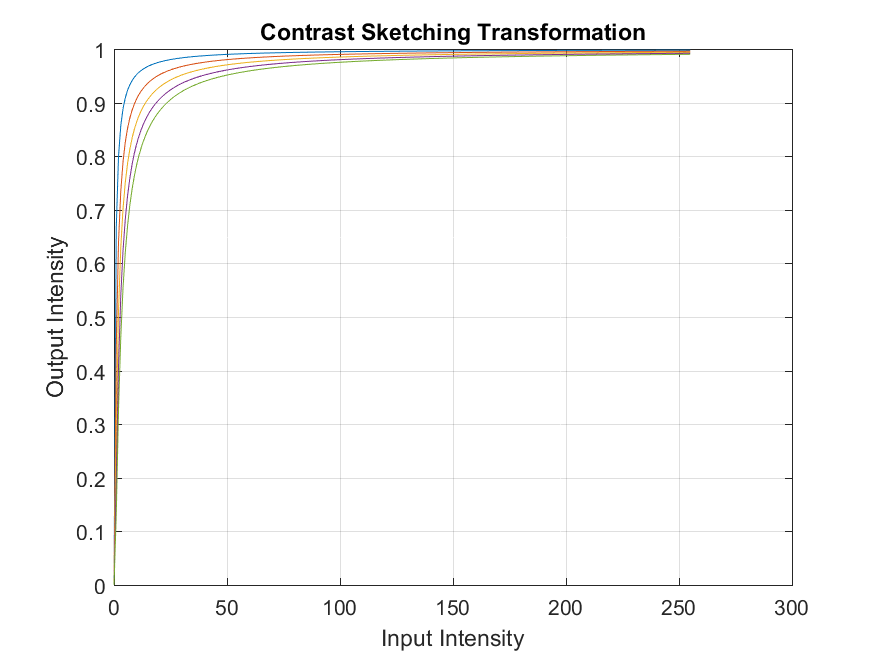
\includegraphics{contrast_stretch}
    \caption{plot}
\end{figure}

\subsection{Constant Offset}

\begin{figure}[H]
    \centering
    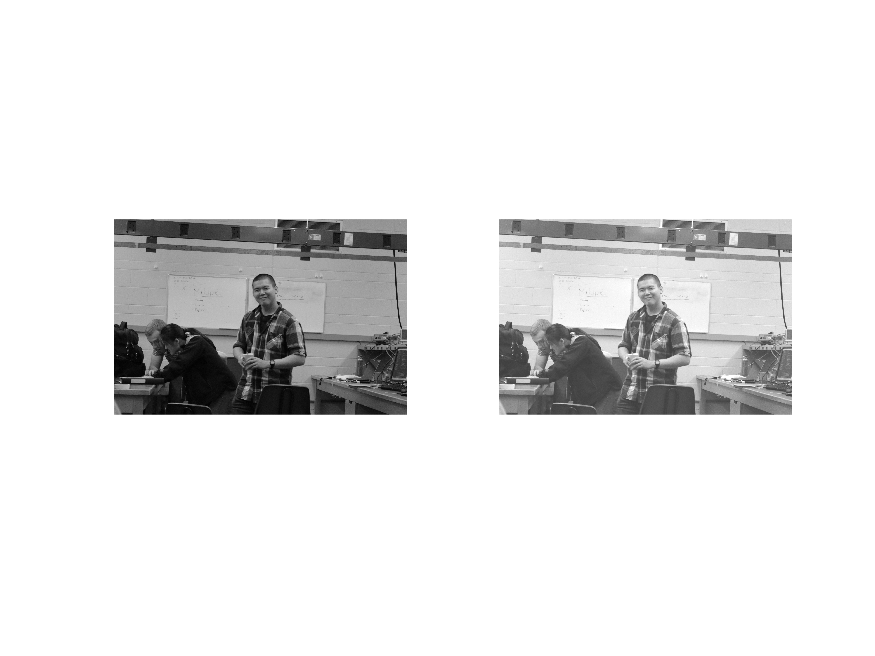
\includegraphics{twoPeters}
    \caption{plot}
\end{figure}

\subsection{Negative Image}

\begin{figure}[H]
    \centering
    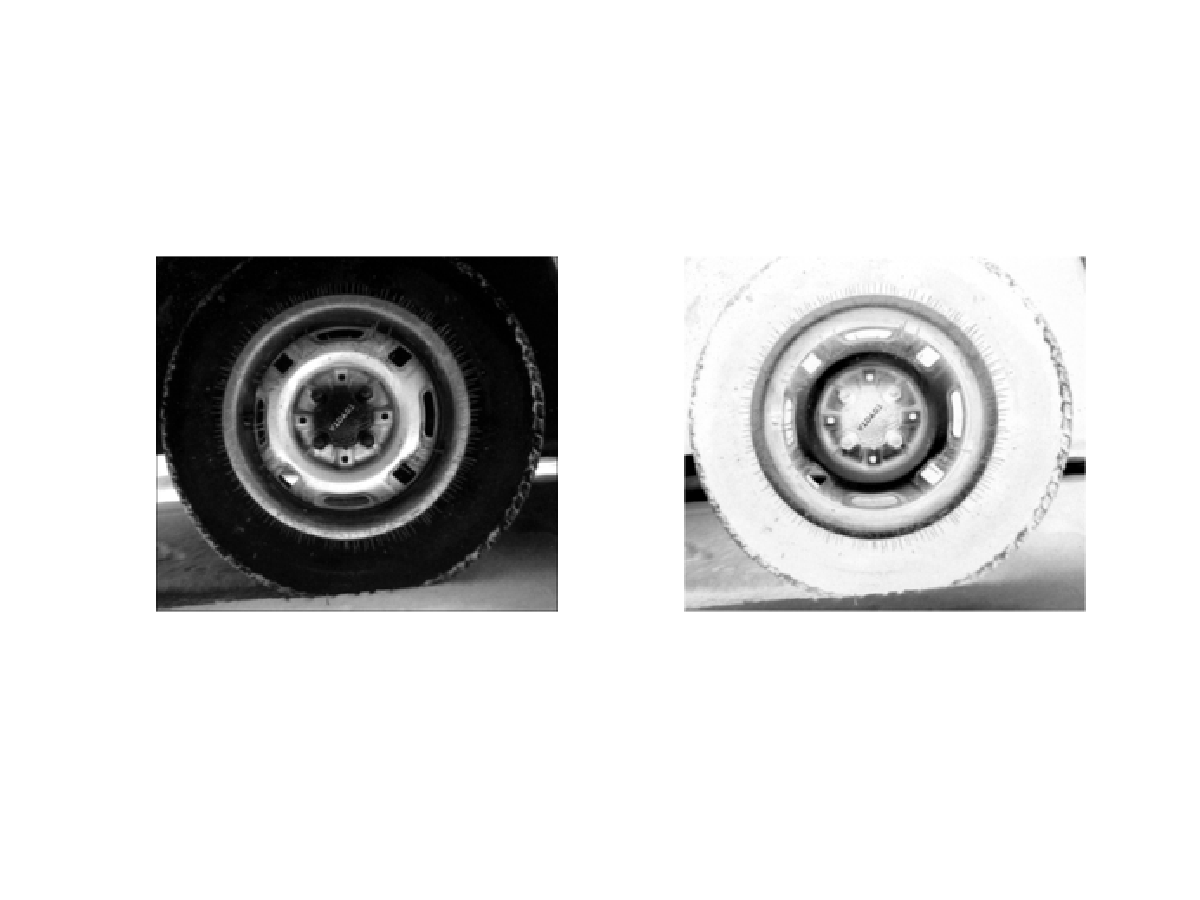
\includegraphics{tire_neg}
    \caption{plot}
\end{figure}

\subsection{Gamma Transform}

\begin{figure}[H]
    \centering
    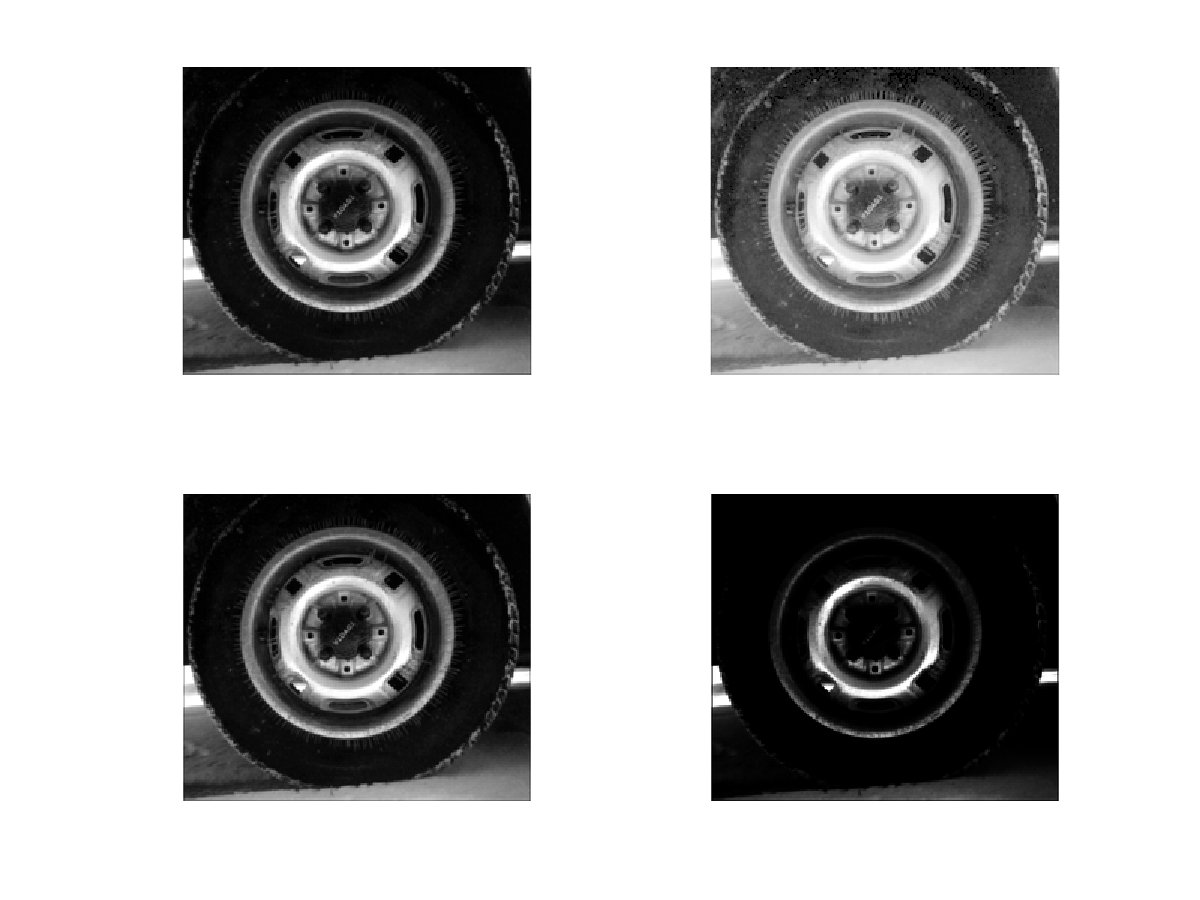
\includegraphics{tire_gamma}
    \caption{plot}
\end{figure}

\subsection{Logarithmic Transfrom}

\begin{figure}[H]
    \centering
    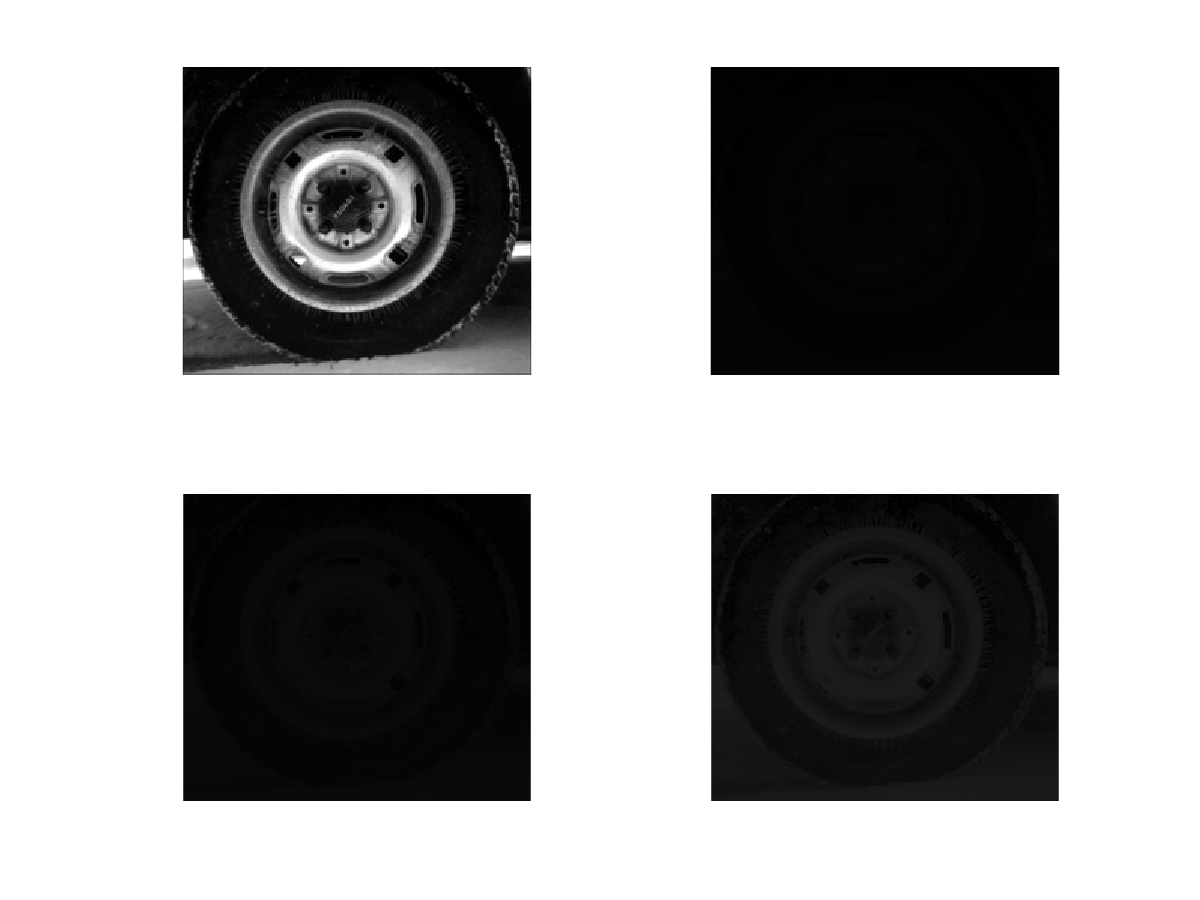
\includegraphics{tire_log}
    \caption{plot}
\end{figure}

\subsection{Piecewise Transform}

\begin{figure}[H]
    \centering
    \includegraphics{piecewise}
    \caption{plot}
\end{figure}

\subsection{Translation}

\begin{figure}[H]
    \centering
    \includegraphics{translation}
    \caption{plot}
\end{figure}
